%%	PST4UserManual.tex
%	Thad Haines		
% 	Purpose:		Document to collect PST v4 changes/information that will end up being a pseudo user manual.
%	Notes:			Build with LuaLatex, use biber as bibliography backend.

\documentclass[12pt]{report}

%% Document Knowns
\newcommand{\CAPTitle}{Power System Toolbox 4 \\
	\vspace{2em}
	--User Manual--\\
	Documentation Version 0.0.0-a.1
}
\newcommand{\Author}{Thad Haines}
\newcommand{\Degree}{-}
\newcommand{\University}{-}
\newcommand{\Year}{2020}
\newcommand{\Subject}{Software Documentation}
\newcommand{\Keywords}{PST, Power System Toolbox, MATLAB, Power system dynamics, AGC, Variable Time Step Integraion}

%%	pretty_preamble.tex
%	Thad Haines		Template
% 	Purpose:		Provide alternative to ugly thesis format.
%	Notes:			Included by thesis main.
%					Build with LuaLatex, use biber as bibliography backend.
%					Bibliography style can be changed below. see ***

%	Alteration History:		10/05/19	Added numbering to paragraphs to mimic subsubsubsections
%							10/11/19	Addition of lscape / pdflscape for landscape possibilities
%							10/17/19	Addition of minted package for purty code~
%							11/21/19	Use of glossaries package implemented.
%							11/30/19	Added siunitx for table formatting


% Tech specific formatting
\usepackage{setspace}
\setlength{\parindent}{0.5in}
\usepackage{indentfirst}
\usepackage{geometry}
\geometry{letterpaper, margin=1in}

%\usepackage{lscape} % for landscape pages
\usepackage{pdflscape} % for landscape pages - rotates digital page so text appears 'normal'

\usepackage{mathrsfs} % for laplace L

\usepackage{comment}
\usepackage{adjustbox}

\usepackage{enumitem} % for alteration of enumerate display 09/21/20

% Glossaries package configuration
\usepackage[nogroupskip, nonumberlist, nopostdot]{glossaries}
\setglossarystyle{long3colheader}
\renewcommand*{\entryname}{Term}
\renewcommand*{\descriptionname}{Definition}
\renewcommand*{\pagelistname}{} % remove page number col
\setlength{\glsdescwidth}{5 in} % width of description - may have to alter
\makeglossaries

% pretty commands for dual build
\newcommand{\fmAddAs}{chapter} % what to add aditional toc as (ugly = parts, pretty = chap)
\newcommand{\MTten}{\footnotesize}
\newcommand{\coverSkip}{2em}
\newcommand{\tocAbstract}{Abstract}
\newcommand{\tocDedication}{Dedication}
\newcommand{\tocAckno}{Acknowledgments}
\newcommand{\tocGlossary}{Glossary of Terms}

%*** Bibliography stuff
\usepackage[backend=biber,style=ieee, % bibliography style may be changed
sorting=nyt, % sorts by author, year, title
autocite=inline, sortcites=true, labelnumber=true, % for compressed cites
dashed=false, % show repeated authors (i.e. don't blank out names)
]{biblatex}
\addbibresource{bibliography.bib}
\nocite{*} % include non referenced citations

% for Altering Section titles to desired compact format.
\usepackage{titlesec} 
\titleformat{\chapter}
{\normalfont\LARGE\bfseries}{\LARGE \thechapter}{20pt}{\LARGE} 

\titlespacing*{\chapter}{0pt}{-30pt}{.25em}
\titlespacing{\section}{0pt}{0pt}{0pt}
\titlespacing{\subsection}{0pt}{0pt}{0pt}
\titlespacing{\subsubsection}{0pt}{0pt}{0pt}
\titlespacing{\bibliography}{0pt}{0pt}{0pt}

% Packages for filler text
\usepackage{blindtext} % for \blindtext -> Loerm ipsum dolor...
\usepackage{lipsum} % for short lines

% for maths and maths symbols
\usepackage{amsmath} 
\usepackage{amssymb}
\usepackage{commath}
\newcommand\numberthis{\addtocounter{equation}{1}\tag{\theequation}} % for simple \numberthis command to add equations to ...

% For list of equations - much pushing around to match other toc,lof...
% Required since list of equations not standard in report format
\usepackage[titles]{tocloft}
\newcommand{\listequationsname}{List of Equations}
\newlistof{thesisequations}{loe}{\listequationsname}
\newcommand{\eqcaption}[1]{
	\addcontentsline{loe}{thesisequations}{%\hspace{1.12em}  
	 \protect\numberline{\theequation} \hspace{1.85em} #1}\par\vspace{-2.5em}}%

%removal of 'chapter change' additional space in lot, lof
\usepackage{xpatch}
\makeatletter
\xpatchcmd{\@chapter}{%
	\addtocontents{lof}{\protect\addvspace{10\p@}}%
	\addtocontents{lot}{\protect\addvspace{10\p@}}%
}{}{}{}
\makeatother

%%% Add Figure zz: to list of figures 
\setlength{\cftfigindent}{0pt}  % remove indentation from figures in lof
\renewcommand{\cftfigaftersnum}{\quad}
\renewcommand{\cftfignumwidth}{4em}

%%% Add Table XX: to list of tables
\renewcommand{\cfttabaftersnum}{\quad}
\setlength{\cfttabindent}{0pt}  % remove indentation from tables in lot
\renewcommand{\cfttabnumwidth}{4em}

% for chapter leader dots
\renewcommand{\cftchapleader}{\cftdotfill{\cftdotsep}}

% For figure usage and linking
\usepackage{graphicx}
\graphicspath{ {figures/} }

% Caption formating footnotesize ~ 10 pt in a 12 pt document
\usepackage[font={footnotesize, bf}]{caption}

% For table formatting
\usepackage{booktabs}
\renewcommand{\arraystretch}{1.2}
\usepackage{floatrow}
\floatsetup[table]{capposition=top} % put table captions on top of tables

% for code listings with color 10/17/19
\usepackage{minted}
\usepackage{xcolor}

% for labeled listings 09/18/20
\usepackage{listings}
\renewcommand\lstlistlistingname{List of Listings} % rename page header
\lstset{basicstyle=\singlespacing,} % basic format of listing...
\makeatletter
\renewcommand*{\l@lstlisting}{\@dottedtocline{1}{0em}{2.3em}} % removing indent from main list of listings
\makeatother

% For header and footer control:
\usepackage{fancyhdr}
\pagestyle{fancy}
\fancyhf{}
\renewcommand{\headrulewidth}{0pt}
\rhead{\thepage}

% Redefine the plain page style so plain pages are same as fancy
\fancypagestyle{plain}{%
	\fancyhf{}%
	\rhead{\thepage}%
	\renewcommand{\headrulewidth}{0pt}% Line at the header invisible
	\renewcommand{\footrulewidth}{0pt}% Line at the footer nonvisible
}

% configurations of counters
\usepackage{chngcntr}
\setcounter{tocdepth}{5} % required to show subsubsections in toc
\setcounter{secnumdepth}{5} % required for x.x.x.x sections % Changed from 3 - 10/5/19

%%% Added for paragraph numbering to be subsubsection
\makeatletter
\renewcommand\paragraph{\@startsection{paragraph}{5}{\z@}%
            {-2.5ex\@plus -1ex \@minus -.25ex}%
            {1.25ex \@plus .25ex}%
            {\normalfont\normalsize\bfseries}}
\makeatother

% Command to correctly add page numbers to toc, lof, lot, loe...
\newcommand{\correctpagenumtoc}[1]{%
	\cleardoublepage
	\phantomsection
	\addcontentsline{toc}{\fmAddAs}{#1}}

% Fix header height
\setlength{\headheight}{15pt}

%%% SI unit x added for tables...
\usepackage[per-mode=fraction]{siunitx} % for si units and num
\sisetup{group-separator = {,}, group-minimum-digits = 3}

\usepackage{array} 		% for >{} column characterisctis
\newcolumntype{L}[1]{>{\raggedright\let\newline\\\arraybackslash\hspace{0pt}}m{#1}}
\newcolumntype{C}[1]{>{\centering\let\newline\\\arraybackslash\hspace{0pt}}m{#1}}
\newcolumntype{R}[1]{>{\raggedleft\let\newline\\\arraybackslash\hspace{0pt}}m{#1}}

% Silence warning that is known to not be a 'thing' when using ieee bibliography
% https://tex.stackexchange.com/questions/451192/file-english-ieee-lbx-not-found-ignoring-mapping-english-english-ieee
\usepackage{silence}
\WarningFilter{biblatex}{File 'english-ieee.lbx'}

% Packages enables content to function as links and describe default pdf behavior
\usepackage[hidelinks]{hyperref}
\hypersetup{
	pdftitle={\CAPTitle},
	pdfauthor={\Author},
	pdfsubject={\Subject},
	pdfkeywords={\Keywords},
	bookmarksnumbered=true,     
	bookmarksopen=true,         
	bookmarksopenlevel=3,       
	colorlinks=false,            
	pdfstartview=Fit,           
	pdfpagemode=UseOutlines,   
	pdfpagelayout=OneColumn
}

%% For including only certain parts of document in build, uncomment :
%\includeonly{frontmatter/glossary} % Optional build modes
\nocite{} 
\newcommand{\tempPB}{\pagebreak \clearpage}
\newcommand{\uglyVspace}{\vspace{-0.75 em}} % used for creating spaces in front matter
\newcommand{\uglyPB}{ }  % used for creating spaces in front matter
\newcommand{\prettyPB}{\pagebreak \clearpage}
\begin{document}
\Large % for cover font size
\begin{titlepage}
	\pagenumbering{roman}
	\setcounter{page}{1}
	\onehalfspacing
	\topskip0pt
	\vspace{4em}
	\vspace*{\fill}
    \begin{center}
        \textbf{\CAPTitle}\\
        \vspace{2em}
        Last Document Build: \today
		\vspace{4em}
		\ \\ % removed by
        \Author \\  
      	\vspace{2em}
		%Last Update: \today
        %A thesis submitted in partial fulfillment of the\\ 
        %requirements for the degree of\\
	%	\vspace{2em}
        %\Degree\\
     %   \vspace{2em}
    %    \vspace{4em}
        %\University\\
        %\Year\\
       % \vspace{.5em}
       % \includegraphics[width=1.25in]{shield.png}
    \end{center}
	\vspace*{\fill}
\end{titlepage}

% Begin roman numbers after cover
\pagestyle{fancy}
\pagenumbering{roman}
\setcounter{page}{2}
\fancyfoot{} % clear footer
\fancyhead[R]{\thepage}

\normalsize
\setlength\parindent{0cm}
\onehalfspacing % for nicer look

%% Front matter
\vspace{2em} % for tech wonkyness
\chapter*{Introduction}
%\addcontentsline{toc}{\fmAddAs}{\tocAbstract}%%% All caps == ugly
% Note the required use of \vspace{1em} to seperate paragraphs.
This is a PST user manual template. BONES!
%\chapter*{Dedication}
\addcontentsline{toc}{\fmAddAs}{\tocDedication}%%% all caps == ugly
\setlength\parindent{0cm}

For you... 
\\And others too.
%\chapter*{Acknowledgments - WIP}
\addcontentsline{toc}{\fmAddAs}{\tocAckno} %%% ugly = ALL CAPS

More officially worded:
\begin{itemize}
\itemsep 0 em
\item Original Creators
\item Known major contributors
\item funding that made \emph{this} work possible.
\end{itemize}


%% Table of contents, lists of tables,figures, equations
% \correctpagenumtoc enables content line to be defined before table or list command is executed
\renewcommand{\contentsname}{Table of Contents \vspace{-.5em}}
\correctpagenumtoc{Table of Contents} 
\tableofcontents

\correctpagenumtoc{List of Tables}
\listoftables

\correctpagenumtoc{List of Figures}
\listoffigures

\correctpagenumtoc{List of Equations}
\listofthesisequations

\onehalfspacing
\chapter*{Glossary of Terms}
\addcontentsline{toc}{\fmAddAs}{\tocGlossary} %%%%
\vspace{-2em}
% There are may be a better way to do this (i.e. use of glossaries package)
% Obviously, A table is used for now.

% using the glossaries package requires the installation of perl.
% additionally, the glossaries package reuires a seperate build of the glossary so that t prints at all (similar to the bibliography using biber)
\renewcommand*{\glsclearpage}{} % remove pagebreak pre-glossary
\renewcommand{\glossarysection}[2][]{} % remove auto glossary title

\newglossaryentry{ACE}{name={ACE}, description={Area Control Error }}
\newglossaryentry{AC}{name={AC}, description={Alternating Current}}
\newglossaryentry{DC}{name={DC}, description={Direct Current}}
\newglossaryentry{PU}{name={PU}, description={Per-Unit}}
\newglossaryentry{SACE}{name={SACE}, description={Smoothed ACE}}
\newglossaryentry{PI}{name={PI}, description={Proportional and Integral}}
\newglossaryentry{PST}{name={PST}, description={Power System Toolbox}}
\newglossaryentry{RACE}{name={RACE}, description={Reported ACE}}
\newglossaryentry{DACE}{name={DACE}, description={Distributed ACE}}
\newglossaryentry{PSS}{name={PSS}, description={Power System Stabilizer }}
\newglossaryentry{AGC}{name={AGC}, description={Automatic Generation Control }}
\newglossaryentry{WECC}{name={WECC}, description={Western Electricity Coordinating Council }}
\newglossaryentry{NERC}{name={NERC}, description={North American Electric Reliability Corporation }}
\newglossaryentry{FERC }{name={FERC}, description={Federal Energy Regulatory Commission }}
\newglossaryentry{EIA}{name={EIA}, description={ United States Energy Information Administration}}
%\newglossaryentry{CTS}{name={CTS}, description={ Classical Transient Stability}}
\newglossaryentry{ODE}{name={ODE}, description={ Ordinary Differential Equation }}
%\newglossaryentry{US}{name={US}, description={United States of America }}
%\newglossaryentry{RTO}{name={RTO}, description={Regional Transmission Organization}}
%\newglossaryentry{ISO}{name={ISO}, description={Independent Service Operator}}
%\newglossaryentry{SI}{name={SI}, description={International System of Units}}
\newglossaryentry{Hz}{name={Hz}, description={Hertz, cycles per second}}
\newglossaryentry{W}{name={W}, description={Watt, Joules per second}}
\newglossaryentry{J}{name={J}, description={Joule, Neton meters, Watt seconds}}
%\newglossaryentry{BES}{name={BES}, description={Bulk Electrical System}}
%\newglossaryentry{BA}{name={BA}, description={Balancing Authority}}
\newglossaryentry{P}{name={P}, description={Real Power}}
\newglossaryentry{Q}{name={Q}, description={Reactive power}}
\newglossaryentry{VAR}{name={VAR}, description={Volt Amps Reactive}}
%\newglossaryentry{IC}{name={IC}, description={Interchange}}
\newglossaryentry{VTS}{name={VTS}, description={Variable Time Step}}
\newglossaryentry{FTS}{name={FTS}, description={Fixed Time Step}}

\glsaddall % so that there is no need to call \gls{label} for each term
\printglossaries


\begin{comment}
% table style glossary for record...

\begin{table}[h]
	\begin{tabular}{@{} p{.25\linewidth} p{.7\linewidth} @{}} %\toprule 
	\textbf{Term} & \textbf{Definition}\\
	%	
	\LaTeX 			& A document preparation system. Favors logical design over visual design. Reportedly widely used in academia... \\
	PSLF 	&	Positive Sequence Load Flow. GE's power system simulation software.\\
	PSDS	&	PSLF Dynamic subsystem.\\
	PSS		&	Power System Stabilizer \\
	AGC		&	Automatic Generation Control \\
	LFC		&	Load Frequency Control \\
	WECC	&	Western Electricity Coordinating Council \\
	NERC	&	North American Electric Reliability Corporation \\
	FERC 	&	Federal Energy Regulatory Commission \\
	PSLTDSim &	Power System Long-Term Dynamic Simulator\\
	LTD		& 	Long-Term Dynamic. May also refer the type of simulation performed by PSLTDSim.\\

	\end{tabular}
\end{table}

\end{comment}


% Body Format
\setlength\parindent{0.5in}
\doublespacing
\pagenumbering{arabic}
\setcounter{page}{1} % Arabic Numbers start at the begining of chapter 1
\setcounter{table}{0}

%% Body of thesis goes here
\chapter{Basic Formatting}
This chapter will show basic formatting of text, figures, tables and equations. It will also be mostly filled with `dummy' text so there is something to look at.

\section{Body Text}
Body text has a $1/2$ inch indent on all paragraphs and double spaced lines.
\lipsum[6]
\section{Figures, In-Text Citations, and Footnotes}
Figure~\ref{fig:athletic logo} is an example of how images can be formatted. Additionally, citations to references will be shown such \cite{latexcompanion}. Footnotes\footnote{This is a footnote text message that doesn't offer much information.} will behave like this\footnote{This is another footnote.}.

\begin{figure}[!ht]
	\centering
	\footnotesize
	
\includegraphics[width=2in]{test/athletic-bw.png}
	\caption{An Athletic logo?}
	\label{fig:athletic logo}
\end{figure}\vspace{-1em} % can be useful to pull following text closer... sometimes, other times messes up format.

A larger graphic example is shown on Page~\pageref{fig:ramp test 1} as Figure~\ref{fig:ramp test 1}. \lipsum[8] 

\begin{figure}[!ht]
	\centering
	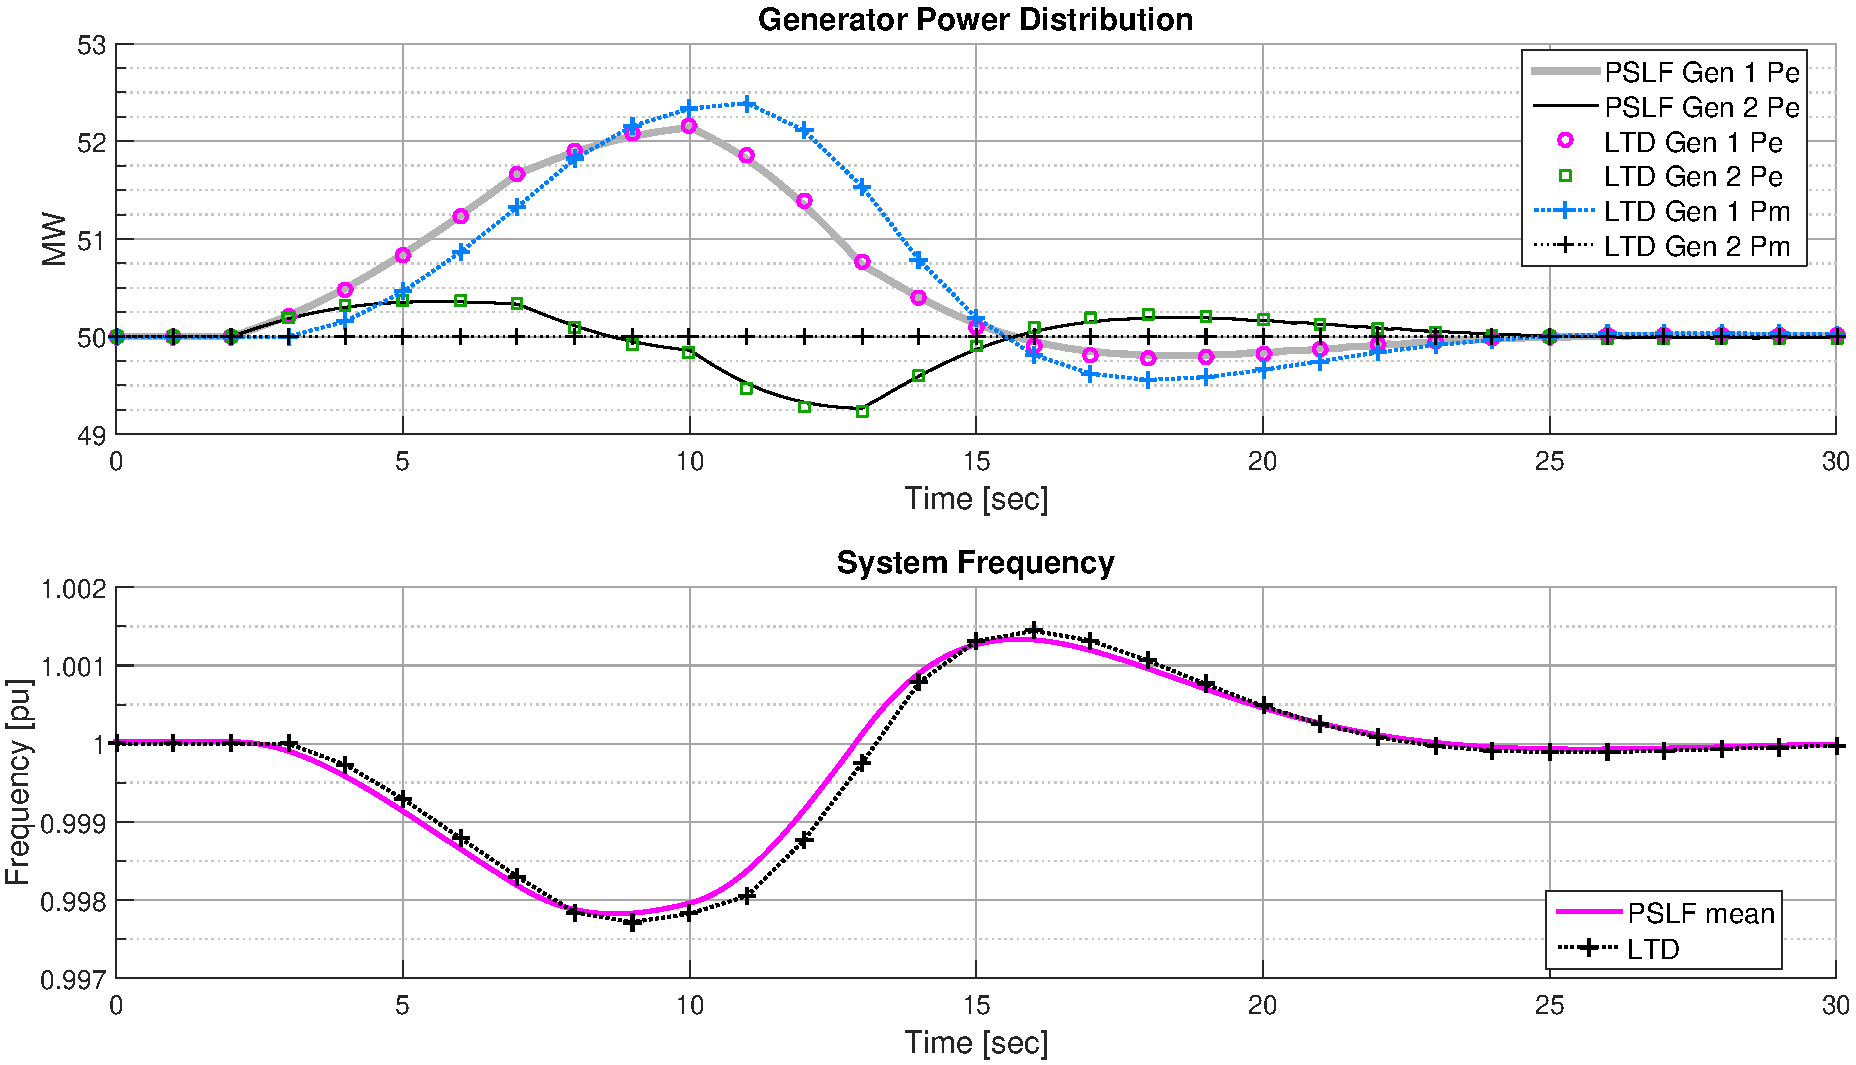
\includegraphics[width=\linewidth]{test/ramp1sec.pdf}
	\caption[60 Second Ramp Test.]{This is a fairly large graphic but can easily be set to any desired width. Additionally, this is a super long caption that would break the table of contents formatting if it weren't for an optional `short title' parameter. There's even a citation in here\cite{stajcar}.}
	\label{fig:ramp test 1}
\end{figure}%\vspace{-1em}

\lipsum[15]

\section{Equations}
	A somewhat fancy equation involving symbols and an integral is pretty easy to put together. \lipsum[5] %
	\begin{equation}{\label{eq:ssSoln}}
		x(t) = \Phi(t) x(0) + \int_{0}^{t}\Phi(t-\tau)Bu(\tau) \text{d}\tau.
	\end{equation}\eqcaption{An example of optional equation captions}

	\lipsum[6]\ Unlike Equation~\ref{eq:ssSoln}, Equation~\ref{eq:one} is pretty basic.%
	\begin{equation}{\label{eq:one}}
		a+b=c
	\end{equation}\eqcaption{.}
	
	Aligned rows of equations are also possible using the \verb|align*| environment and a custom \verb|numberthis| command. The following math is very math.
	\begin{align*}
		G(\$) &= \dfrac{20}{\$(\$+5)(\$+10)}\\
		\zeta = 0.59116 &, \Phi_M = 58.59\\
		\therefore \omega_{\Phi_M} &= \omega \angle -121.41^\circ\\
		\text{From Bode: } \omega_{\Phi_M} &= 1.9 \\
		\abs{\omega_{\Phi_M}} &= -14.3 \\
		\therefore K &= 10^\frac{14.3}{20} =5.188 \text{ abs} \numberthis \label{eq:align}
	\end{align*}\eqcaption{Some Gain Calculation}

\section{Tables}
Tables can look like Table~\ref{tab:exp1}. Notice the slimming effect of no vertical lines\ldots .
 Quisque vehicula, urna sed
ultricies auctor, pede lorem egestas dui, et convallis elit erat sed nulla. Donec luctus. 

\begin{table}[h]
	\centering
	\begin{tabular}{@{} l r r r r @{}} 	
		\toprule % @ signs to remove extra L R space
		\footnotesize % this will make the table font 10pt
		& \multicolumn{1}{c}{Experiment 1}	& \multicolumn{1}{c}{Experiment 2}	& \multicolumn{1}{c}{Experiment 3}	& \multicolumn{1}{c}{Experiment 4} \\
		\midrule
		Old	& 29.631	& 17.333	& 222.999	& 11.222 \\
		Not Old	& 54.321	& 166.233	& 556.123	& 54.666 \\
		Almost New	& 118.791 &	54.289 &	445.321 &	88.122 \\
		New& 	222.897	& 10.000 &	777.000	 & 90.100 \\
		\bottomrule
	\end{tabular}
	\caption{An example table with no vertical lines.}
	\label{tab:exp1}
\end{table}

Table style may be altered to a slightly different style if it seems appropriate.  Quisque vehicula, urna sed
ultricies auctor, pede lorem egestas dui, et convallis elit erat sed nulla. Donec luctus. 
Notice that chapters start on a new page.

Tables may also be input vai a single command incase it seems more logical...

% Testing of external table build for \input later
\begin{singlespace}
\begin{table}[H]
	\centering
	\begin{tabular}{@{} l l l  @{}} 	
		\toprule % @ signs to remove extra L R space
		\footnotesize % this will affect the table font (makse it 10pt)
		\raggedright % for non justified table text
		Method	&		Result & Absolute Error		\\
		\midrule		
%
%Step Input Low Pass Example
%time step:  0.50
%Method: Trapezoidal Int	 Absolute Error from calculated
Calculated& 	1.750083866&	0.000000000\\
Exact& 	1.750082530&	0.000001336\\
RK4&	1.680138966&	0.069944900\\
solve\_ivp& 	1.719657220	&0.030426646\\
lsim&	1.671851297&	0.078232568\\
%
		\bottomrule
	\end{tabular}
	\caption{Trapezoidal integration results a of low pass filter using a $t$ step of 0.5.}
	\label{tab: trap lowpass res}
\end{table}
\end{singlespace}
	
	


\chapter{Chapters and Sections}
This chapter is used only to show nesting of sections and space around chapter and section headings.

\section{First Section}
This is the First Section. It will have two sub sections. %%%
 Quisque vehicula, urna sed
ultricies auctor, pede lorem egestas dui, et convallis elit erat sed nulla. Donec luctus. 

\subsection{First SubSection}
This is the first... %%%
 Quisque vehicula, urna sed
ultricies auctor, pede lorem egestas dui, et convallis elit erat sed nulla. Donec luctus. 


\subsubsection{A subsubsection}
This is a fairly nested sentence. %%%
 Quisque vehicula, urna sed
ultricies auctor, pede lorem egestas dui, et convallis elit erat sed nulla. Donec luctus. 

\subsubsection{The second subsubsection}
Seems like going any deeper than a subsubsection could be a bit much, but is possible to configure \LaTeX\ to number paragraphs like sections if required.
%%%

\subsection{Second Subsection}
This is the second. This subsection will actually have another subsection in it.%%%
  Quisque vehicula, urna sed
 ultricies auctor, pede lorem egestas dui, et convallis elit erat sed nulla.

\section{Second Section}
A second section. %%%
 Quisque vehicula, urna sed
ultricies auctor, pede lorem egestas dui, et convallis elit erat sed nulla. Donec luctus. Curabitur
et nunc. 

\section{Third Section}
A third Section. %%%
 Quisque vehicula, urna sed
ultricies auctor, pede lorem egestas dui, et convallis elit erat sed nulla. Donec luctus. Curabitur
et nunc. 

\chapter{Bibliography}
\onehalfspacing
\printbibliography[heading=none]

% Appendix format
\appendix
\doublespacing

%% appendicies go here
\chapter{TEMPORARY: Formatting Examples}
%%% Ugly version requires Appendix A:, seems redundant in pretty version

%% Blow up counters for toc, lo(tfe) style examples. Probably not useful in real thesis

\setcounter{figure}{66}
\setcounter{table}{13}
\setcounter{equation}{41}
This appendix is included to show how appendices work, blowing up of numbering, and to also serve as an easy \LaTeX\ formatting template. Despite this being an appendix, it is still numbered like a chapter.

\section{Numberings in Equations}
Additionally, a reminder of Ohm's law
\begin{equation}{\label{eq:ohms law} }
V = IR
\end{equation}\eqcaption{Ohm's Law} % this function creates a new paragraph.
\noindent shows that equation numbering has blown up. This is to show spacing on the table of contents.
 
\section{Numberings in Tables}
Table~\ref{tab:exp2} is full of nonsense data and is numbered artificially large.

\begin{table}[!ht] % use H to turn into a float...
	\centering
	\begin{tabular}{@{} lllll @{}} 	
		\toprule % @ signs to remove extra L R space
		\footnotesize % this will affect the table font (makse it 10pt)
		One& Two  & Three  & Four  & Five  \\
		\midrule		
		2.35& 45.87  & 9.00  & 1.00  &0.33  \\
		5.88& 48.01  & 7.85  & 2.35  & 0.45 \\
		\bottomrule
	\end{tabular}
	\caption{Another Table.}
	\label{tab:exp2}
\end{table}

\section{Numberings in Figures}
Finally, Figure~\ref{fig: boxcat} shows how figure numbers look when double digit.

\begin{figure}[!ht]
	\centering
	\footnotesize
	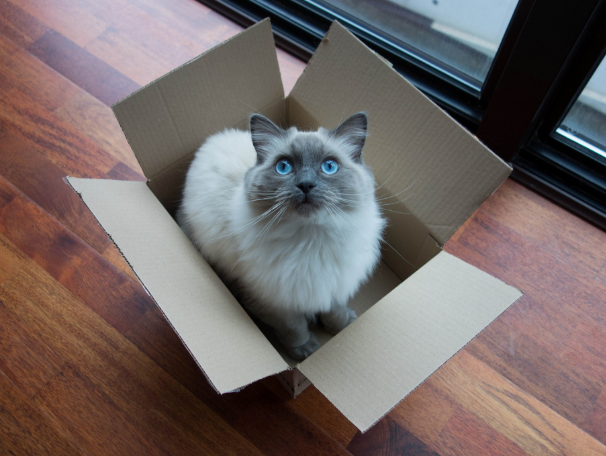
\includegraphics[height=1.5in]{test/boxcat}
	\caption{A boxcat in its natural environment.}
	\label{fig: boxcat}
\end{figure}\vspace{-1em} % will remove 1 white space after image - typically good

\section{Code using Minted}
Code can be added using the \verb|minted| package. The example below is for a Python example, but can be configured other ways. Note that a \verb|--shell-escape| command had to be added to the \TeX Studio build command due to peculiarities with the package. 
Additionally, the \verb|minted| \LaTeX\ package requires python to be installed with the \verb|pygments| package.
This can be done via the '\verb|py -m pip install -U pygments|' console command.

\begin{figure}[!ht]
\begin{minted}[
frame=lines,
framesep=2mm,
baselinestretch=1.2,
bgcolor=gray!13,
fontsize=\footnotesize,
linenos
]{python}
def sumPe(mirror):
    """Returns sum of all electrical power from active machines"""
    sysPe = 0.0

    # for each area
    for area in mirror.Area:
        # reset current sum
        area.cv['Pe'] = 0.0

        # sum each active machine Pe to area agent
        for mach in area.Machines:
            if mach.cv['St'] == 1:
                area.cv['Pe'] += mach.cv['Pe']

        # sum area agent totals to system
        sysPe += area.cv['Pe']

    return sysPe
\end{minted}
	\centering
	\footnotesize
	\caption{Code listing as a figure.}
	\label{fig: codeTest}
\end{figure}\vspace{-1em} % will remove 1 white space after image - typically good

Other packages exist for code insertion, but they may or may not be as pretty. Remember, as with anything, this is totally optional and voluntary...

\pagebreak
\section{Labeled Code Listing}
Sometime you might want to label code as listing - like a person may in \ref{lst: rando code}.
\begin{lstlisting}[caption={Some MATLAB code},label={lst: rando code},language=MATLAB]
for n=1:length(ts)
    
    % Handle basic generation curve
    if ts(n) >= 30 && ts(n) < 90
        % up ramp
        % use first 1/4 cycle of a sin to ramp up
        xs(n) = maxGen*sin( (ts(n)-30) * 2*pi/240); 
    elseif ts(n) >= 150 && ts(n) < 210
        % down ramp
        % use second 1/4 cycle of a sin to ramp down
        xs(n) = maxGen*sin( (ts(n)-150) * 2*pi/240 + pi/2);   
    elseif ts(n) >= 90 && ts(n) < 150
        % held peak
        xs(n) = maxGen;
    else
        % no generation
        xs(n) = 0;
    end
    
    % Handle Cloud cover generation reductions
    if ts(n) >= 45 && ts(n) < 55
        xs(n) = maxGen*.2;
    elseif ts(n) >= 120 && ts(n) < 140
        xs(n) = xs(n)*0.7;
    elseif ts(n) >= 180 && ts(n) < 190
        xs(n) = xs(n)*0.85;
    end
    
end
\end{lstlisting}


\pagebreak
Of course, the listing format may not be very `great', so, a listing environment can precede a minted block to get the best of both yeah?
I mean, if Listing \ref{lst: code 2} is an example then like, yeah.

\begin{lstlisting}[caption={Empty listing before a minted block},label={lst: code 2},language=MATLAB]
\end{lstlisting}\vspace{-2 em}
\begin{minted}[
frame=lines,
framesep=2mm,
baselinestretch=1.2,
bgcolor=gray!13,
fontsize=\footnotesize,
%linenos
]{Matlab}
for n=1:length(ts)
    
    % Handle basic generation curve
    if ts(n) >= 30 && ts(n) < 90
        % up ramp
        % use first 1/4 cycle of a sin to ramp up
        xs(n) = maxGen*sin( (ts(n)-30) * 2*pi/240); 
    elseif ts(n) >= 150 && ts(n) < 210
        % down ramp
        % use second 1/4 cycle of a sin to ramp down
        xs(n) = maxGen*sin( (ts(n)-150) * 2*pi/240 + pi/2);   
    elseif ts(n) >= 90 && ts(n) < 150
        % held peak
        xs(n) = maxGen;
    else
        % no generation
        xs(n) = 0;
    end
    
    % Handle Cloud cover generation reductions
    if ts(n) >= 45 && ts(n) < 55
        xs(n) = maxGen*.2;
    elseif ts(n) >= 120 && ts(n) < 140
        xs(n) = xs(n)*0.7;
    elseif ts(n) >= 180 && ts(n) < 190
        xs(n) = xs(n)*0.85;
    end
    
end
\end{minted}

Right? I mean ideally this should look really good.

 % formatting examples

\end{document}